% !TeX root = ./Dyplom.tex
% chktex-file 21

\chapter{Ocena skuteczności modeli}
	Analizowane algorytmy są nienadzorowane, co oznacza, że nie ma jednoznacznej metody oceny wyników.
	Jedyną metodą ewaluacji modeli tematycznych dającą pewność jest manualna weryfikacja poprzez np.\ ocenianie w trzystopniowej skali,
		które reprezentacje tematów są spójne, a które nie.
	Jest to jednak kosztowna metoda, dlatego tworzy się algorytmy dające dobre przybliżenie ocen człowieka.
	Ocena spójności tematów według takich algorytmów porównywana jest z ocenami człowieka poprzez współczynnik korelacji Pearsona.

	Alternatywną metodą zaproponowaną w~\cite{Word_intrusion} jest podmiana słowa w reprezentacji tematu (ang.\ \emph{word intrusion task}).
	W wygenerowanych zestawach słów podmieniane jest jedno słowo na losowe.
	Następnie uczestnicy badania muszą zidentyfikować podmienione słowo.
	Jeśli tematy są spójne, to niepasujące słowo powinno być łatwe do zidentyfikowania,
		natomiast w mniej spójnych tematach słowa będą sprawiały wrażenie bardziej losowych, co utrudni poprawne rozwiązanie problemu.

\section{Ewaluacja spójności reprezentacji tematów}
	Najpopularniejszą metodą ewaluacji wygenerowanych tematów jest analiza reprezentacji tematów (zbioru słów opisujących temat).
	Im lepiej słowa opisujące temat reprezentują wszystkie dokumenty w danym temacie, tym lepszy model.
	W pracy~\cite{U_MASS} autorzy proponują algorytm (zwany dalej \(C_{UMass}\))
		analizujący pary słów z reprezentacji tematu pod kątem współwystępowania w dokumentach korpusu.
	Jeśli para słów często występuje razem w dokumentach, to są one powiązane.
	Można więc określić spójność całej reprezentacji tematu badając wszystkie w niej zawarte pary słów.
	Miara ta porównana została z wynikami zadania podmiany słowa i uzyskała ona lepszą korelację z ocenami ludzi.

	Autorzy~\cite{C_NPMI} proponują rozwiązanie bazujące na wektorach kontekstowych słów tematu (zwane dalej \(C_{NPMI}\)).
	Wektory te są obliczane na podstawie współwystępujących słów w kontekście analizowanego słowa.
	Kontekst jest definiowany jako tzw.\ przesuwne okno (ang.\ \emph{sliding window}) zwierające \(\pm 5\) otaczających słów.
	Następnie wektory są ważone algorytmem NPMI (ang.\ \emph{Normalized Point Mutual Information}).
	Końcowa wartość obliczana jest jako średnia odległość kosinusowa między wszystkimi parami wektorów kontekstowych słów tematu.

	W pracy~\cite{Eval_Topics} autorzy stworzyli bazową strukturę pozwalającą na zdefiniowanie metryk \(C_{UMass}\), \(C_{NPMI}\)
		oraz innych miar spójności w jednej przestrzeni.
	W projekcie skorzystano z biblioteki \verb|Gensim|\footnote{\url{https://radimrehurek.com/gensim/models/coherencemodel.html} (dostęp dnia 29 maja 2021)},
		która implementuje miary spójności na podstawie tych definicji.

\section{Ewaluacja spójności rozkładu tematów}
	Ze względu na specyfikę korpusu możliwe jest również sformułowanie metryki wykorzystującej porządek obrad sejmu.
	Każde posiedzenie przebiega zgodnie z ustaloną strukturą, gdzie marszałek zarządza obrady na temat danej ustawy, poprawki czy interpelacji,
		a następnie kolejni posłowie wyrażają swoją opinię na ten temat.
	Można więc założyć, że w obrębie debaty nad jednym punktem obrad, wypowiedzi powinny zostać zakwalifikowane do tego samego zbioru tematycznego.
	Stworzono więc algorytm wykorzystujący tę zależność, przedstawiony na listingu~\ref{lst:consistency_alg}.
	Implementacja algorytmu w języku Python pokazana jest na listingu~\ref{lst:score_consistency}.
	Założono, że w zdecydowanej większości przypadków, kolejne dwie wypowiedzi powinny mieć przypisany ten sam temat.

	Algorytm analizuje osobno każdy dzień posiedzeń.
	Wypowiedzi sortowane są zgodnie z kolejnością wynikającą z transkrypcji przemówień.
	Jeśli w ciągu dnia jest mniej niż dwie wypowiedzi, to dzień jest pomijany.
	W zbiorze danych występuje jeden taki przypadek, natomiast mediana wynosi 138.
	Wśród wypowiedzi danego dnia porównywane są tematy par sąsiadujących wypowiedzi.
	Zliczane są zarówno znalezione pasujące pary, jak i różniące się.
	Jeśli temat analizowanej wypowiedzi jest nieznany (algorytm HDBSCAN nie przypisał dokumentu do żadnej grupy),
		to jest ona pomijana.
	Mechanizm ten zapobiega sytuacji, w której duża liczba nieprzypisanych dokumentów zawyżałaby wynik.
	Dzieje się tak ze względu na to, że nieprzypisane dokumenty często stanowią znaczną część zbioru (30--50\%),
		przez co istnieje duże prawdopodobieństwo znalezienia par takich dokumentów.
	Dodatkowo, od sumy różniących się par odejmowana jest liczba o 1 mniejsza od liczby tematów danego dnia.
	Działanie to rekompensuje przejścia między tematami, które muszą wystąpić i nie są błędem.
	Takich przejść w ciągu dnia wystąpi co najmniej tyle, ile jest tematów minus jeden.
	Końcowy wynik obliczany jest jako stosunek zgadzających się par do wszystkich zliczonych par.
	
	\begin{lstlisting}[style=algorithm,label=lst:consistency_alg,caption=Algorytm obliczania spójności tematów]
input: speeches sorted by original order of speaking, with date and assigned topic identifier
output: consistency score between 0 and 1 with higher score indicating more consistent topics
	
same_per_day := []
different_per_day := []

for each speeches in data grouped by date do
	if len(speeches) < 2
		continue
	
	same := 0
	different := 0
	for i in range(len(speeches) - 1) do
		if speeches[i].topic is unknown
			continue

		if speeches[i].topic = speeches[i + 1].topic
			same := same + 1
		else
			different := different + 1

	topic_count := len(speeches.topic.unique())
	different := different - (topic_count - 1)
	
	same_per_day.append(same)
	different_per_day.append(different)

score = sum(same_per_day) / sum(same_per_day, different_per_day)
return score
	\end{lstlisting}

\section{Końcowa ocena}
	Powyższe metody nie poddają ocenie samej liczby tematów i liczby nieprzyporządkowanych dokumentów.
	Z tego powodu, wysoki wynik mógłby osiągnąć model, który znalazłby zaledwie 5 tematów.\todo{Pokazać jakieś dane-rysunek albo tabelka}
	Taki model przyporządkuje wszystkie dokumenty generując bardzo ogólne tematy.
	Podobnie wysoki wynik osiągnie model, który wygeneruje tysiące bardzo szczegółowych tematów.
	Takie modele można odfiltrować definiując odpowiednie progi, jednak taka metoda wymusza ustanowienie założeń,
		które niekoniecznie będą optymalne.
	Zamiast tego, stworzone zostały dwie dodatkowe miary: jedna ocenia liczbę przyporządkowanych dokumentów \(s_f\), druga ocenia liczbę tematów \(s_T\).
	Końcowa ocena modelu jest średnią ocen \(C_{UMass}\), \(s_c\), \(s_f\), \(s_T\)\todo{ustalić końcowy zestaw} przeskalowanych do pełnego zakresu (0, 1).
	Skalowanie odbywa się przy pomocy klasy \verb|MinMaxScaler| z biblioteki \verb|scikit-learn|,
		jak przedstawiono w linijce 18 listingu~\ref{lst:final_score}.

	\subsection{Ocena liczby przyporządkowanych dokumentów}\label{sec:score_not_found}
		Miara oceniająca liczbę przyporządkowanych dokumentów korzysta bezpośrednio z wyniku grupowania.
		Grupa oznaczona jako '-1' oznacza dokumenty, które nie zostały zgrupowane, a więc nie mają przypisanego tematu.
		Rozmiar tej grupy odejmowany jest od rozmiaru korpusu uzyskując liczbę dokumentów z rozpoznanymi tematami.
		Liczba ta dzielona jest przez rozmiar korpusu, co daje miarę w przedziale (0, 1).
		Działanie to przedstawione jest w linijce 16 listingu~\ref{lst:final_score},
			gdzie \verb|scores['not_found']| to kolumna tabeli zawierająca rozmiar grupy nieprzyporządkowanych dokumentów dla każdego modelu.
		\todo{jakiś rysunek czy coś}

	\subsection{Ocena liczby tematów}
		Dużo trudniej jest ocenić liczbę tematów, gdyż zarówno osiemdziesiąt ogólnych tematów,
			jak i tysiąc szczegółowych mogą zostać uznane za odpowiednie.
		Zważając jednak na specyfikę korpusu, przyjęto że różnorodność poruszanych kwestii powinna skutkować relatywnie dużą liczbą tematów.
		Z tego powodu uznano, że zbyt ogólne tematy nie są odpowiednie w tym kontekście.
		Nadmiernie szczegółowe, a więc o małej liczebności tematy również tracą informacje o zależnościach między dokumentami,
			więc także uznane zostały za niepożądane.
		W takim wypadku za odpowiednią liczbę tematów przyjęto medianę liczby tematów dla wszystkich testowanych modeli, która wyniosła 219.

		W celu określenia wyniku każdego modelu wykorzystano zmodyfikowaną standaryzację Z.
		Standaryzacja Z obliczana jest zgodnie z następującym wzorem:
		\[z=\frac{x-\mu}{\sigma}\]
		gdzie:
		\begin{itemize}
			\item \(x\) wartość zmiennej,
			\item \(\mu\) średnia z populacji,
			\item \(\sigma\) odchylenie standardowe populacji.
		\end{itemize}
		
		Średnia arytmetyczna i odchylenie standardowe są jednak podatne na wpływ wartości leżących daleko od średniej.
		Z tego powodu często wykorzystywana jest zmodyfikowana standaryzacja Z, która mierzy odległości od mediany:
		\[\tilde{z}=\frac{x-\tilde{x}}{k\cdot MAD}\]
		gdzie:
		\begin{itemize}
			\item \(x\) wartość zmiennej,
			\item \(\tilde{x}\) mediana z populacji,
			\item \(k=1.486\) wartość korekcyjna stanowiąca przybliżenie odchylenia standardowego,
			\item \(MAD\) średnie odchylenie bezwzględne --- \(median\left(|x_i-\tilde{x}|\right)\).
		\end{itemize}

		Tak ustandaryzowane dane rozłożone są wokół zera, gdzie liczby tematów mniejsze od mediany mają ujemny wynik, a większe dodatni.
		Takie odległości interpretowane są jako odległości od najlepszej liczby tematów,
			im większa odległość tym gorszy powinien być wynik takiego modelu.
		Aby wyrazić te odległości w skali (0, 1), gdzie 1 to najlepszy wynik, znormalizowano dane
			poprzez odwrócenie wartości bezwzględnej standaryzacji Z powiększonej o 1 (aby minimalna wartość była równa 1):
		\[s_T=\frac{1}{|\tilde{z}|+1}\]
		Implementacja tej miary przedstawiona została na listingu~\ref{lst:final_score} jako funkcja \verb|modified_zscore|.
		\todo{rys}

	\subsection{Implementacja}
		Algorytmy zaimplementowane zostały w języku Python.
		Wykorzystane zostały biblioteki \verb|numpy|, \verb|pandas|, \verb|scikit-learn| oraz \verb|scipy|.

	\begin{lstlisting}[label=lst:score_consistency,language=Python,caption=Funkcja obliczająca spójność s\_c]
def score_consistency(df: pd.DataFrame) -> float:
	same_per_day = []
	different_per_day = []

	for _, day in df.sort_values('speech_order').groupby(by='date'):
		if len(day) < 2:
			continue

		same = 0
		different = 0
		for i in range(len(day) - 1):
			if day.iloc[i].topic == -1:
				continue

			if day.iloc[i].topic == day.iloc[i + 1].topic:
				same += 1
			else:
				different += 1

		topics = len(day.topic.unique())
		different -= (topics - 1)

		same_per_day.append(same)
		different_per_day.append(different)

	s_c = np.sum(same_per_day) / np.sum([*same_per_day, *different_per_day])

	return s_c
		\end{lstlisting}

		\begin{lstlisting}[label=lst:final_score,language=Python,caption=Obliczanie finalnej oceny spójności tematów dla listy modeli]
from sklearn.preprocessing import MinMaxScaler
from scipy import stats
import numpy as np

def modified_zscore(x: List[float]) -> List[float]:
	median = np.median(x)
	deviation_from_med = x - median

	mad = np.median(np.abs(deviation_from_med))

	consistency_correction = 1.4826
	mod_zscore = deviation_from_med / (consistency_correction * mad)

	return mod_zscore

scores['s_f'] = [(total - x) / total for x in scores['not_found']]

scores['s_T'] = 1 / (np.abs(modified_zscore(scores['topic_count'])) + 1)

scaler = MinMaxScaler()
minimax = scaler.fit_transform(scores[['s_c','u_mass','s_f','s_T']])

scores['avg'] = np.nanmean(minimax, axis=1)
		\end{lstlisting}

\section{Porównanie z LDA}
	Tematy uzyskane metodą BERTopic zostały porównane z popularną metodą analizy tematycznej --- LDA\@.
	W tym celu wykonano pomiary spójności algorytmami opisanymi w poprzednich rozdziałach.
	Jedną z zasadniczych wad algorytmu LDA jest fakt, iż liczba tematów jest jego parametrem.
	Aby znaleźć optymalną liczbę tematów, przeprowadzono pomiary dla różnych wartości parametru z zakresu [10--300].
	Dokumenty przetworzono tą samą metodą, co w przypadku generowania wektorów TF-IDF w rozdziale~\ref{sec:tfidf_vectors},
		mianowicie lematyzacja słownikami \emph{Morfeusz2}, usunięcie polskich słów bez znaczenia (ang.\ \emph{stop words}) oraz wygenerowanie bigramów.
	Ze względu na ograniczenia techniczne związane z pamięcią operacyjną maszyny (128GB), analizie poddano sto tysięcy losowo wybranych dokumentów,
		co stanowi ok.~34\% całości korpusu.
	Wyniki tych pomiarów przedstawione są na rysunku~\ref{fig:lda_scores} oraz w tabeli~\ref{tab:lda_scores}.
	Z danych można odczytać, że dokładność modelu utrzymuje się na podobnym poziomie do ok.~80 tematów, potem zaczyna gwałtownie spadać.
	Za optymalną liczbę tematów wybrano więc 80 ze względu na zróżnicowanie korpusu, który z pewnością zawiera dużo tematów.

	\begin{figure}[htb]
		\centering
		\begin{minipage}{.5\textwidth}
			a)\par\medskip % chktex 10
			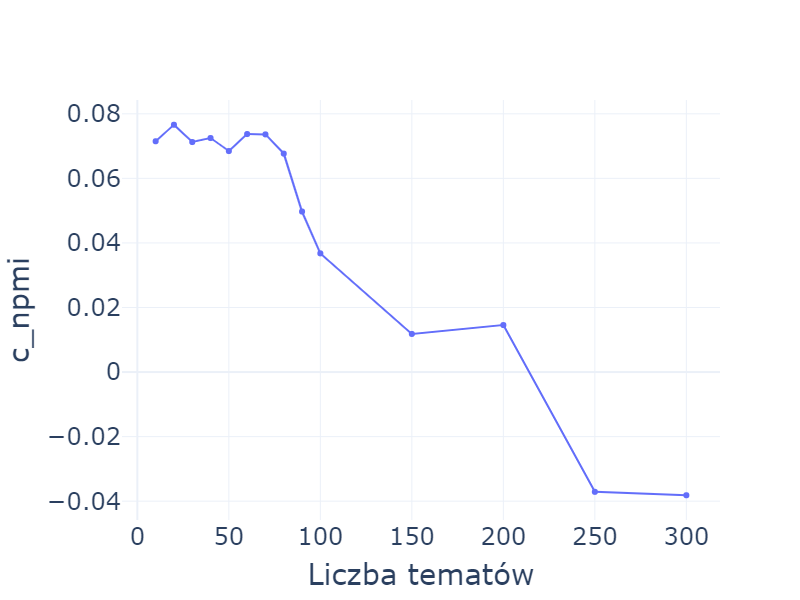
\includegraphics[width=\linewidth]{rys05/lda_c_npmi.png}
		\end{minipage}%
		\begin{minipage}{.5\textwidth}
			b)\par\medskip % chktex 10
			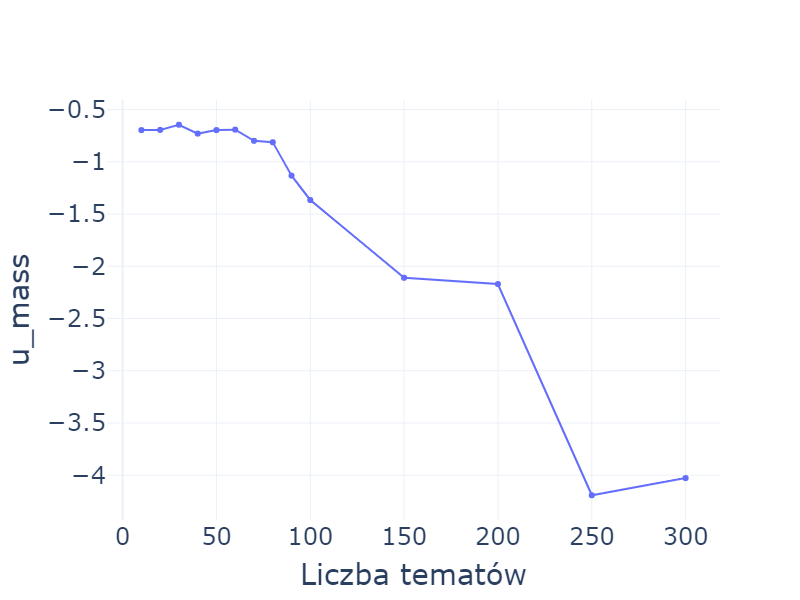
\includegraphics[width=\linewidth]{rys05/lda_u_mass.png}
		\end{minipage}
		\caption{Wyniki pomiarów dla LDA:\ a) \(C_{NPMI}\), b) \(C_{UMass}\)}\label{fig:lda_scores} % chktex 9 chktex 10
	\end{figure}

	\begin{table}[htb]
		\centering
		\caption{Wyniki pomiarów dla LDA w zależności od liczby tematów}\label{tab:lda_scores}
		\begin{tabular}{lrr}
			\toprule
			{} &    c\_npmi &    u\_mass \\
			\midrule
			10  &  0.071499 & -0.696868 \\
			20  &  0.076610 & -0.694938 \\
			30  &  0.071255 & -0.645520 \\
			40  &  0.072496 & -0.730301 \\
			50  &  0.068460 & -0.696550 \\
			60  &  0.073730 & -0.692332 \\
			70  &  0.073619 & -0.799463 \\
			80  &  0.067665 & -0.813064 \\
			90  &  0.049716 & -1.132477 \\
			100 &  0.036761 & -1.366198 \\
			150 &  0.011804 & -2.110305 \\
			200 &  0.014556 & -2.170508 \\
			250 & -0.037109 & -4.191849 \\
			300 & -0.038166 & -4.027447 \\
			\bottomrule
			\end{tabular}			
	\end{table}

	Dla znalezionych tematów wygenerowano reprezentacje składające się z pięciu najwyżej ocenianych słów.
	Losowo wybrane 5 tematów przedstawiono w tabeli~\ref{tab:lda_topics}a.
	Dodatkowo, ze względu na to, iż mediana liczby znalezionych tematów algorytmem HDBSCAN wyniosła 219,
		postanowiono zbadać również model LDA dla 200 tematów (tabela~\ref{tab:lda_topics}b).
	Dla obu tych modeli widoczny jest problem opisany w rozdziale~\ref{sec:topic_modeling}.
	Mianowicie, reprezentacje tematów zawierają wiele podobnych słów specyficznych dla całego korpusu, a nie tematu (,,ustawa'', ,,minister'', czy ,,poseł'').
	Podjęto próby poszerzenia listy słów nieinformatywnych, jednak szybko okazało się, iż takich słów jest zbyt wiele
		--- po usunięciu słów specyficznych dla korpusu nadal reprezentacje tematów składały się często ze słów typu ,,czas'', ,,kwestia'', ,,chodzi''.
	Nie stwierdzono zauważalnej różnicy między dokładnością reprezentacji wygenerowanych dla 80 tematów, a tymi dla 200.
	
	\begin{table}[htb]
		\caption{Reprezentacje pięciu losowo wybranych tematów dla LDA:\ a) 80 tematów, b) 200 tematów}\label{tab:lda_topics} % chktex 9 chktex 10
		\centering
		a) % chktex 10
		\begin{tabularx}{.7\textwidth}{rl}
			\toprule
			A	&	rok | mieć | europejski | minister | r	\\ 
			B	&	państwo | ustawa | mieć | rok | Polska	\\ 
			C	&	minister | państwo | dziecko | rok | szkoła	\\
			D	& minister | poseł | pytanie | mieć | chcieć	\\
			E	& ustawa | mieć | poseł | wysoki | poprawka	\\
			\midrule
		\end{tabularx}

		b) % chktex 10
		\begin{tabularx}{.7\textwidth}{rl}
			A	&	ustawa | projekt | ustawy | komisja | wysoki	\\ 
			B	&	rok | mieć | minister | poseł | Maryja \\ 
			C	&	ustawa | zmiana | projekt | prawo | ustawy \\
			D	&	trybunał | konstytucyjny | ustawa | rok | Trybunału	\\
			E	&	ustawa | mieć | rok | Pan | sprawa	\\
			\bottomrule
		\end{tabularx}
	\end{table}
